    \newcommand\n{5}
    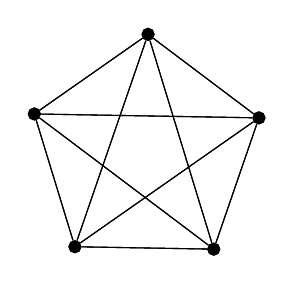
\begin{tikzpicture}
        \tikzstyle{point}=[circle,thick,draw=black,fill=black,inner sep=0pt,minimum width=4pt,minimum height=4pt]

        \begin{scope}[rotate=17]
        %the multiplication with floats is not possible. Thus I split the loop in two.
        \foreach \number in {1,...,\n}{
            \node[point] (N-\number) at ({\number*(360/\n)}:1.5cm) {};
        }

        \foreach \number in {1,...,\n}{
            \foreach \y in {1,...,\n}{
                \draw (N-\number) -- (N-\y);
            }
        }
        \end{scope}
    \end{tikzpicture}
